% siminos/reversal/Bernoulli.tex      pdflatex LC21; bibtex LC21
% temporary: siminos/spatiotemp/chapter/LC21Bernoulli.tex
% $Author: predrag $ $Date: 2021-12-24 01:25:20 -0500 (Fri, 24 Dec 2021) $

\section{A fair coin toss}
\label{s:coinToss}
\renewcommand{\ssp}{\ensuremath{x}}               % state space point

The very simplest example of a deterministic law of evolution that gives
rise to `chaos' is the {\em Bernoulli} map, \reffig{fig:BernPart}\,(a),
which models a
\HREF{https://www.random.org/coins/?num=2&cur=40-antique.aurelian} {coin
toss}. Starting with a random initial state, the map generates,
deterministically,  a sequence of tails and heads with the 50-50\%
probability.

We introduce the model in its conventional, time-evolution dynamical
formulation, than reformulate it as a lattice field theory, solved by
enumeration of all admissible \emph{{\lattstate}s}, field configurations that
satisfy a  global fixed point condition, and use this simple setting to
motivate
(1) the \emph{fundamental fact}: for a given lattice period, the {\em
\HillDet} of stabilities of global solutions counts their number
(\refsect{sect:fundFact}), and
(2) the {\tzeta} counts their translational symmetry group orbits
(\refsect{s:zeta1D}).

\subsection{Bernoulli map} %Doubling map}
\label{s:Bernoulli}
%ChaosBook return to
% \example{Bernoulli shift map \statesp\ partition.}{ \label{exam:BernMap}

%\renewcommand{\statesp}{state space}
%\renewcommand{\Statesp}{State space}
%\renewcommand{\stateDsp}{state-space}
%\renewcommand{\StateDsp}{State-space}

%
%%%%%%%%%%%%%%%%%%%%%%%%%%%%%%%%%%%%%%%%%%%%%%%%%%%%%%%%%%%%%
\begin{figure}
  \centering
{(a)}
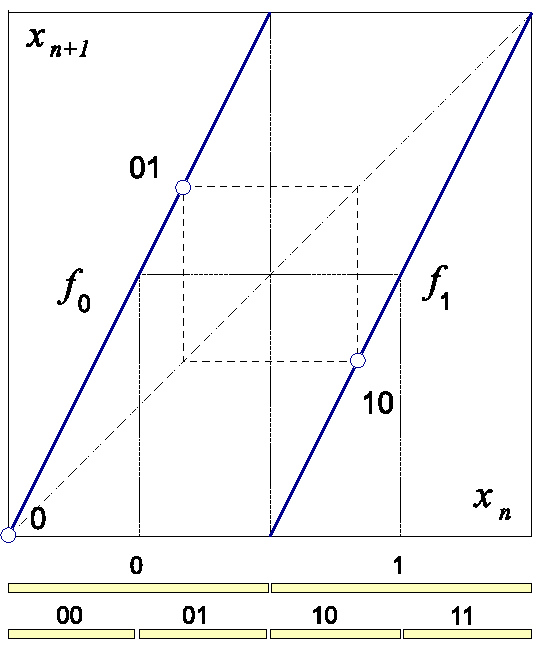
\includegraphics[width=0.35\textwidth]{BernPartCL18}
~~~
{(b)}$\!\!\!\!$
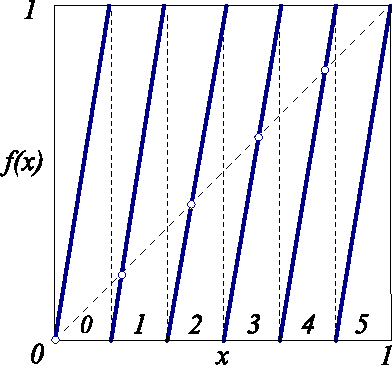
\includegraphics[width=0.40\textwidth]{fig_d_2CL18}

  \caption{\label{fig:BernPart}
(Color online)~~~
(a)
The `coin toss' map \refeq{BerShift}, together with the
$\cycle{0}$ fixed point, and the \cycle{01} 2-cycle. Preimages
of the critical point $\ssp_c=1/2$ partition the unit interval into
$\{\pS_0,\pS_1\}$, $\{\pS_{00},\pS_{01},\pS_{10},\pS_{11}\}$, $\dots$,
subintervals.
(b)
The base-${s}$ Bernoulli map, here with the `dice throw' stretching parameter ${s}=6$,
partitions the unit interval into $6$ subintervals $\{\pS_{\Ssym{}}\}$,
labeled by the ${6}$-letter alphabet \refeq{base-sAlph}. As the map is a
circle map, $\ssp_{5}=1=0=\ssp_{0} \quad(\mbox{mod}\;1)$.
          }
\end{figure}
%%%%%%%%%%%%%%%%%%%%%%%%%%%%%%%%%%%%%%%%%%%%%%%%%%%%%%%%%%%%%%
%

The base-2 {\em Bernoulli} shift map,
\index{Bernoulli!shift}
\index{shift!Bernoulli}
\beq
\ssp_{\zeit+1} =
% \flow{}{\ssp_{\zeit}} =
\left\{ \begin{array}{ll}
        f_0(\ssp_{\zeit}) =  2 \ssp_{\zeit} \,, \quad
                                    & \ssp_{\zeit} \in \pS_0=[0,1/2) \\
        f_1(\ssp_{\zeit}) =  2 \ssp_{\zeit} \;\; (\mbox{mod}\;1)\,, \quad
                                    & \ssp_{\zeit} \in \pS_1 =[1/2,1)
         \end{array}\right.
\,,
\ee{BerShift}
is shown in \reffig{fig:BernPart}\,(a).
If the linear part of such map has an integer-valued slope,
or `stretching' parameter $s\geq2$,
\beq
\ssp_{\zeit+1} \,=\, {s} \ssp_{\zeit}
\ee{BerStretch}
that maps state $\ssp_{\zeit}$ into a state in the `extended \statesp',
outside the unit interval,
the $(\mbox{mod}\;1)$ operation results in the base-${s}$ Bernoulli
circle map,
\renewcommand{\ssp}{\ensuremath{\phi}}             % lattice site field
\beq
\ssp_{\zeit+1}
% = \flow{}{\ssp_{\zeit}}
= {s} \ssp_{\zeit}
\;\; (\mbox{mod}\;1)
%    \,,\qquad \qquad \ssp_{\zeit}\in [0,1)
\,,
\ee{n-tuplingMap}
sketched as a \HREF{https://www.random.org/dice/}{dice throw} in
\reffig{fig:BernPart}\,(b).
The $(\mbox{mod}\;1)$ operation subtracts
$\Ssym{\zeit}=\left\lfloor{s}\ssp_{\zeit}\right\rfloor$, the integer part of ${s}
\ssp_{\zeit}$, or the circle map \emph{winding number}, to keep
$\ssp_{\zeit+1}$ in the unit interval $[0,1)$, and partitions the unit
interval into ${s}$ subintervals $\{\pS_\Ssym{}\}$,
\beq
\ssp_{\zeit+1}
% = \flow{}{\ssp_{\zeit}}
% = \hflow{}{\ssp_{\zeit}} - \Ssym{\zeit+1}
= {s} \ssp_{\zeit} - \Ssym{\zeit}
\,,\qquad  \ssp_{\zeit}\in\pS_{\Ssym{\zeit}}
\,,
\ee{circ-m}
where $\Ssym{\zeit}$ takes values in the ${s}$-letter alphabet
\beq
\Ssym{} \in \A=\{0,1,2,\cdots,s-1\}
\,.
\ee{base-sAlph}

The Bernoulli map is a highly instructive example of a
hyperbolic dynamical system. Its symbolic dynamics is simple:
the base-${s}$ expansion of the initial point $\ssp_0$ is also its
temporal itinerary, with symbols from alphabet \refeq{base-sAlph}
indicating that at time $\zeit$ the orbit visits the subinterval
$\pS_{\Ssym{\zeit}}$. The map is a `shift':
a multiplication by ${s}$ acts on the base-${s}$
representation of $\ssp_{0}=.\Ssym{1}\Ssym{2}\Ssym{3}\cdots $ (for
example, binary, if ${s}=2$) by shifting its digits,
\bea
\ssp_{1}
    &=& \map(\ssp_{0})
    =.\Ssym{2}\Ssym{3}\cdots
%\continue
%\ssp_{\Ssym{2}\Ssym{3}\cdots}
%    &=& \shift{}\,\ssp_{\Ssym{1}\Ssym{2}\Ssym{3}\cdots}
\,.
\label{shiftBern}
\eea

Periodic points can be counted by observing that the preimages of
critical points $\{\ssp_{c1},\ssp_{c2},\cdots\ssp_{c,s-1}\}$ =
$\{{1}/s,{2}/s,\cdots,(s-1)/s\}$ partition the unit interval into
$\{\pS_0,\pS_1,\cdots,\pS_{s-1}\}$, $\{\pS_{\Ssym{1}\Ssym{2}}\}$, $\dots$,
$s^\cl{}$ subintervals, each containing {\em one}  unstable
period-$\cl{}$ periodic point
$\ssp_{\Ssym{1}\Ssym{2}\cdots\Ssym{\cl{}}}$, with stability multiplier
${s}^\cl{}$, see \reffig{fig:BernPart}. The Bernoulli map is a
full shift, in the sense that every itinerary is \admissible, with one
exception: on the circle, the rightmost fixed point is the same as the
fixed point at the origin, $\ssp_{s-1}=\ssp_{0}\quad(\mbox{mod}\;1)$,
so these fixed points are identified and counted as one, see
\reffig{fig:BernPart}. The total number of periodic points of period
$\cl{}$ is thus
\beq
N_{\cl{}} = s^{\cl{}} - 1
\,.
\ee{noPerPtsBm}


\subsection{Temporal Bernoulli}
\label{s:1D1dLatt}

To motivate our formulation of a \spt\ chaotic field theory to be
developed below, we now recast the local initial value, time-evolution
Bernoulli map problem as a \emph{temporal lattice} fixed point condition,
the problem of enumerating and determining all global solutions.

`Temporal' here refers to the lattice site field  $\ssp_\zeit$ and the
source (winding number) $\Ssym{\zeit}$ taking their values on the lattice
sites of a 1\dmn\ \emph{temporal} integer lattice $\zeit\in\integers$.
Over a finite lattice segment, these can be written compactly  as a
\emph{{\lattstate}} and the corresponding \emph{symbol \brick}
\beq
\transp{\Xx} % = \{\ssp_j\}
             = (\ssp_{\zeit+1},\cdots,\ssp_{\zeit+\cl{}})
\,,\quad
\transp{\Mm} % = \{\Ssym{j}\}
             = (\Ssym{{\zeit+1}},\cdots,\Ssym{{\zeit+\cl{}}})
\,,
\ee{pathBern}
where $\transp{(\cdots)}$ denotes a transpose.
The Bernoulli equation \refeq{circ-m}, rewritten as a first-order
difference equation
% \refeq{LC21:1dBernLatt}
\beq
-\ssp_{\zeit+1} + {s}\ssp_{\zeit} - \Ssym{\zeit} =0
\,,\qquad  \ssp_{\zeit} \in [0,1)
\,,
\ee{1stepDiffEq}  % called {...1dBernLatt} elsewhere
takes the matrix form
\beq
\jMorb\,\Xx - \Mm =0
\,,\qquad
\jMorb =  - {\shift} + {s}\id
% former \ee{tempBernFix}
\,,
\ee{tempBern}
where the $[\cl{}\!\times\!\cl{}]$ matrix
\beq
\shift_{jk}=\delta_{j+1,k}
\,,\qquad
\shift
=  \left(\begin{array}{ccccc}
             0    &  1    &        &   &  \cr
                  &  0    &   1    &   &  \cr
                  &       &        & \ddots &  \cr
                  &       &        & 0 & 1 \cr
             1    &       &        &   & 0
          \end{array} \right)
\,,
\ee{hopMatrix}
implements the shift operation \refeq{shiftBern}, a cyclic permutation
that translates for\-ward-in-time {\lattstate} $\Xx$ by one site,
$\transp{(\shift \Xx)}=(\ssp_2,\ssp_3,\cdots,\ssp_\cl{},\ssp_1)$. The
time evolution law \refeq{circ-m} must be of the same form for all times,
so the {\shiftOp} $\shift$ has to be time-translation invariant, with
$\shift_{\cl{}+1,\cl{}}=\shift_{1\cl{}}=1$ matrix element enforcing the
periodicity. After $\cl{}$ shifts, a {\lattstate} returns to the initial
state,
\beq
\shift^\cl{}=\id
\,.
\ee{shift2n}

As the {temporal Bernoulli} condition \refeq{tempBern} is a linear
relation, a given \brick\ $\Mm$, or `code' in terms of alphabet
\refeq{base-sAlph}, corresponds to a unique temporal {\lattstate} $\Xx$.
That is why Percival and Vivaldi\rf{PerViv} refer to such symbol \brick\
$\Mm$ as a {\em linear code}.

\subsection{Bernoulli as a continuous time dynamical system}
\label{s:bernODE}

The discrete time derivative of a lattice configuration \Xx\ evaluated at the
lattice site \zeit\ is given by the {difference operator}\rf{Elaydi05}
    \index{lattice!derivative}\index{derivative, lattice}
    \index{lattice!derivative, forward}\index{difference operator}
\beq
\dot{\ssp}_\zeit =
\left[\frac{\partial\Xx}{\partial\zeit}\right]_\zeit
        =
    \frac{\ssp_{\zeit+1} - \ssp_{\zeit}}{\Delta\zeit}
\,.
\ee{lattTimeDer}
The {temporal Bernoulli} condition \refeq{tempBern} %{1stepDiffEq}
can be thus viewed as a time-discretized, first-order ODE dynamical
system
\beq
   \dot{\Xx} \,=\, \vel(\Xx) \,,
\ee{1stepVecEq}
where the `velocity' vector field $\vel$ is given by
\[
\vel(\Xx) \,=\,
   % \vel(\Xx;\Mm) \,=\,
(s-1)\,\Xx-\Mm
\,,
\]
with the time increment set to $\Delta\zeit=1$, and perturbations that
grow (or decay) with rate $({s}-1)$. By inspection of
\reffig{fig:BernPart}\,(a), it is clear that for \emph{shrinking},
${s}<1$  parameter values the orbit is stable for\-ward-in-time, with a
single linear branch, 1-letter alphabet $\A=\{0\}$, and the only
{\lattstate}s being the single fixed point  $\ssp_0=0$, and its repeats
$\Xx=(0,0,\cdots,0)$. However, for \emph{stretching},  ${s}>1$  parameter
values, the Bernoulli system (more generally, R{\'e}nyi's beta
transformations\rf{Renyi57}) that we study here, every {\lattstate}
$\Xx_\Mm$ is unstable, and there is a {\lattstate} for each admissible
symbol \brick\ \Mm.
    %
    \PC{2021-08-23} {
    Should we include ``Quotienting the temporal Bernoulli system''
    \refeq{1stepDiffEqBlog}?
    }


\bigskip

\noindent\textbf{A fair coin toss, summarized.}
We refer to the \emph{global} temporal lattice condition \refeq{tempBern}
as the `\emph{temporal} Bernoulli', in order to distinguish it from the
one-time step Bernoulli evolution \emph{map} \refeq{n-tuplingMap}, in
preparation for the study of \emph{\spt} systems to be undertaken in
\refref{CL18}. In the lattice formulation, a \emph{global} {temporal
{\lattstate}} $\Xx_\Mm$ is determined by the requirement that the
\emph{local} temporal lattice condition \refeq{1stepDiffEq} is satisfied
at every lattice site. In \spt\ formulation there is no need for
for\-ward-in-time, close recurrence searches for the returning periodic
points. Instead, one determines each global {temporal {\lattstate}}
$\Xx_\Mm$ at one go, by solving the fixed point condition
\refeq{tempFixPoint}. The most importantly for what follows, the \spt\
field theory of \refref{CL18}, this calculation requires no recourse to any
\emph{explicit coordinatization and partitioning of system's state
space}, and \emph{no explicit symbolic dynamics}.
    \PC{2020-12-17}{
Link to the ChaosBook. Maybe refer to \AW.
    }

%%%%%%%%%%%%%%%%%%%%%%%%%%%%%%%%%%%%%%%%%%%%%%%%%%%%%%%%%%%%%%%%%%%%%%%
%\renewcommand{\statesp}{phase space}
%\renewcommand{\Statesp}{Phase space}
%\renewcommand{\stateDsp}{phase-space}
%\renewcommand{\StateDsp}{Phase-space}
